\documentclass[10 pt,a4paper, openany]{article}
%titlepage
\usepackage[hidelinks]{hyperref}
\usepackage[italian]{babel}
\usepackage[T1]{fontenc}
\usepackage[utf8x]{inputenc}
\usepackage{amsfonts}
\usepackage{multicol}
\usepackage{graphicx}
\usepackage{amsmath}
\usepackage{framed}
\usepackage{extarrows}
\usepackage{cancel}
\usepackage{eurosym}
\usepackage{listingsutf8}
\usepackage{lastpage}
\usepackage{rotating} 
\usepackage{multirow}
\usepackage{placeins}

\usepackage{caption}
\usepackage{makecell}
\usepackage{longtable}
\usepackage{array}
\date{}


\usepackage{makeidx}
\makeindex
\usepackage{fancyhdr}
\pagestyle{fancy}
\lhead{
\includegraphics[width=.6cm]{../../../../../file_comuni/immagini/obelisk_sample_02.png}
  Obelix Group}
\chead{}
\rhead{\rightmark }% \leftmark}%da rimettere
\lfoot{}
\cfoot{}
\rfoot{\thepage / \pageref*{LastPage}}
%%%%%%%%%%%%%%%%%%%%%%%%%%%%%%%%%%%%%%
%\usepackage{lipsum}
\usepackage{../../../../../file_comuni/copertina2}
\nomedoc{Verbale interno 2017-05-22}
\versione{v1\_0\_0}
\datacreazione{2017/05/22}
\verifica{Riccardo Saggese}
\approvazione{Nicolò Rigato}
\redazione{Emanuele Crespan \eanche Federica Schifano}
\uso{interno}
\distribuzione{Prof. Tullio Vardanega \eanche Prof. Riccardo Cardin \eanche Red Babel \eanche Gruppo Obelix}
\sommario{Verbale dell'incontro tra i membri del gruppo \emph{Obelix} in data 2017-05-22}


\begin{document}
\paginatitolo
\section{Informazioni sulla riunione}

\begin{itemize}
\item[] Data: 2017-05-22
\item[] Luogo: Torre Archimede - Via Trieste, 63 Padova
\item[] Ora: 14:00
\item[] Durata: 115'
\item[] Partecipanti interni: Obelix
  \begin{itemize}
  \item[] Emanuele Crespan
  \item[] Federica Schifano
  \item[] Nicolò Rigato
  \item[] Riccardo Saggese
  \item[] Silvio Meneguzzo
  \item[] Tomas Mali
 \end{itemize}
\end{itemize}

\section{Argomenti trattati}
\begin{enumerate}
	\item Uso git-flow	
	\item Punto della situazione RP max
	\item 

	
\end{enumerate}


\section{Decisioni Prese}
\begin{enumerate}
	\item E' stato deciso di usare git-flow per una più corretta gestione della repo, e per una migliore suddivisione del lavoro controllando il flusso dei dati ed evitando possibili "casini" tramite l'utilizzo delle feature.
	E' stato stilato un insieme di regole per l'utilizzo basilare e corretto di git-flow, presentiamo un breve riassunto dei comandi principali (data una repo già inizializzata correttamente con git-flow): 
	\begin{itemize}
		\item git clone ssh://user@host/path/to/repo.git
		\item git checkout -b develop origin/develop (copia del develop all'interno della propria repo locale)
		\item git flow feature start MYFEATURE  (creato un branch partendo dal develop)
		\item git flow feature finish MYFEATURE (fine della propria feature e merge nel develop)
	\end{itemize}
	Dopodiché si è aggiornata la seguente repository includendo il lavoro sviluppato fino ad oggi
	
	\item Si è svolta una rapida rivisitazione delle idee concettuali sviluppate riguardanti l'SDK e la Demo e si è iniziata la stesura più approfondita dell'architettura, con dei diagrammi di flusso dei dati (per confermare anche l'idea generale e il collegamento tra i vari componenti) e con successiva stesura di ulteriori classi e metodi.
	Qua presentiamo il flusso dei dati sviluppati in formato grezzo:
	
		\FloatBarrier
		\begin{figure}[ht]
			\centering
			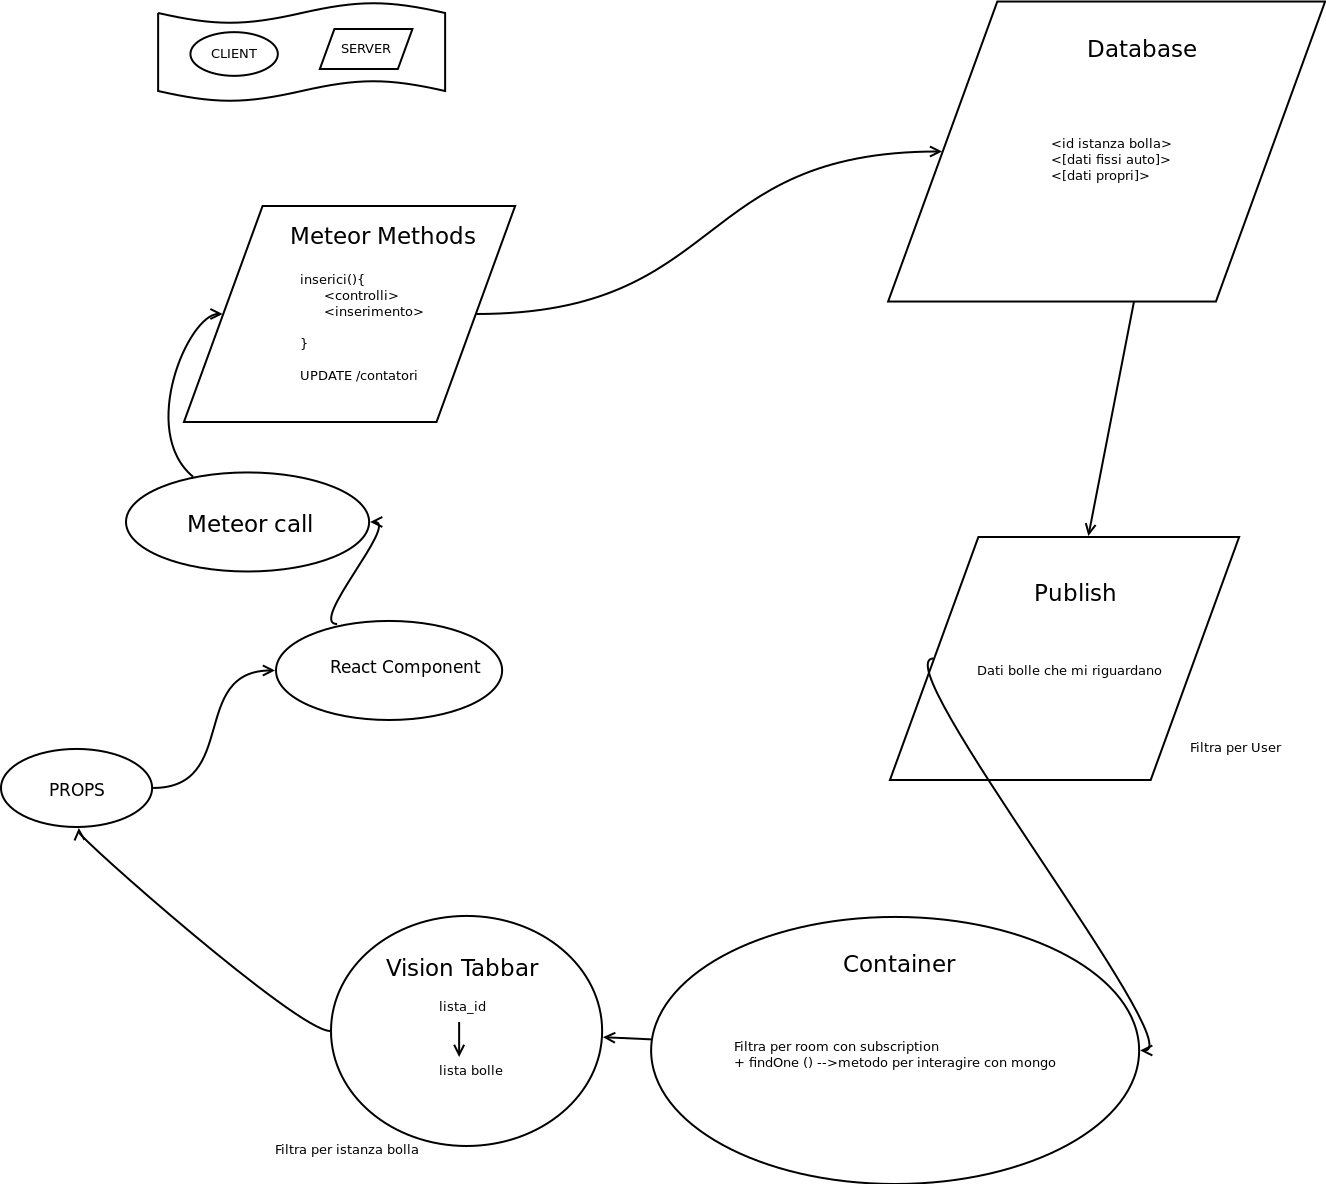
\includegraphics[scale=0.30]{img/flussoD.png}
			\caption{schema flusso dati}
		\end{figure}
	
\end{enumerate}


\end{document}